\documentclass[12pt,a4paper]{report}
\usepackage[utf-8]{inputenc}
\usepackage[margin=1in]{geometry}
\usepackage{graphicx}
\usepackage{amsmath}
\usepackage{amssymb}
\usepackage{fancyhdr}
\usepackage{float}
\usepackage{hyperref}
\usepackage{listings}
\usepackage{xcolor}
\usepackage{setspace}
\usepackage{caption}
\usepackage{subcaption}

\onehalfspacing
\pagestyle{fancy}
\fancyhf{}
\rhead{\thepage}
\lhead{COVID-19 Mathematical Modeling}

\title{
    \textbf{\Large COVID-19 Pandemic Dynamics: \\
    A Comprehensive Mathematical Modeling Study}
    \\ \vspace{0.5cm}
    \large Stability Analysis and Sensitivity Investigation
}

\author{
    \textbf{Team Members:} \\[0.3cm]
    Mohd Usham (ECE/23125/1173) \\
    Ritik Aryan (ECE/23134/1182) \\
    Rishabh Kumar (ECE/231233/1181) \\
    Shashi Prakash Yadav (CSE/23/1144) \\[0.5cm]
    \textbf{Project Mentor:} \\[0.3cm]
    Prof. Sudeshna Mondal
}

\date{\today}

\begin{document}

% Title Page
\maketitle

\newpage
\tableofcontents
\newpage

% ============================================================================
\chapter{Introduction}
% ============================================================================

\section{Background}

The COVID-19 pandemic has significantly impacted global health systems and economies. Mathematical modeling provides crucial insights into disease transmission dynamics, helping predict outbreak trajectories and evaluate intervention strategies. This study presents a comprehensive mathematical model based on compartmental disease dynamics with vaccination and hospitalization components.

\section{Objectives}

The primary objectives of this research are:

\begin{enumerate}
    \item To develop a comprehensive SVEIHIR compartmental model for COVID-19 transmission
    \item To analyze disease-free equilibrium (DFE) stability and endemic equilibrium behavior
    \item To identify bifurcation points and determine critical transmission parameters
    \item To perform sensitivity analysis on key model parameters
    \item To evaluate the effectiveness of vaccination strategies
    \item To examine the impact of transmission rate variations on disease dynamics
\end{enumerate}

\section{Significance}

Understanding pandemic dynamics through mathematical models enables:
\begin{itemize}
    \item Prediction of disease spread patterns
    \item Evaluation of intervention strategies
    \item Resource allocation optimization
    \item Policy decision support
    \item Risk assessment and preparedness planning
\end{itemize}

% ============================================================================
\chapter{Mathematical Model and Methodology}
% ============================================================================

\section{Model Formulation}

The model considers a population stratified into six compartments:
\begin{itemize}
    \item $S(t)$: Susceptible individuals
    \item $V(t)$: Vaccinated individuals
    \item $I_1(t)$: Asymptomatic infected individuals
    \item $I_2(t)$: Symptomatic infected individuals
    \item $H(t)$: Hospitalized individuals
    \item $R(t)$: Recovered individuals
\end{itemize}

\section{System of Differential Equations}

The dynamics are governed by the following system of ODEs:

\begin{equation}
\begin{aligned}
\frac{dS}{dt} &= \Lambda - (\beta_1 I_1 + \beta_2 I_2)S - dS - q_1 S + \eta R \\
\frac{dI_1}{dt} &= (\beta_1 I_1 + \beta_2 I_2)S - q_2 I_1 - \kappa I_1 - \alpha I_1 - d I_1 \\
\frac{dI_2}{dt} &= \kappa I_1 - (\phi_1 + \phi_2)I_2 - (d + \mu_1)I_2 \\
\frac{dH}{dt} &= \phi_1 I_2 - \psi H - (d + \mu_2)H \\
\frac{dR}{dt} &= \alpha I_1 + \phi_2 I_2 + \psi H - dR - \eta R \\
\frac{dV}{dt} &= q_1 S + q_2 I_1 - d V
\end{aligned}
\end{equation}

\section{Parameter Definitions}

\subsection{Table 1: Model Parameters from Literature}

\begin{center}
\begin{tabular}{|c|c|c|}
\hline
\textbf{Parameter} & \textbf{Value} & \textbf{Description} \\
\hline
$\Lambda$ & $6.5 \times 10^4$ & Birth/recruitment rate (persons/day) \\
$\beta_1$ & $1 \times 10^{-10}$ & Asymptomatic transmission rate \\
$\beta_2$ & $0.413 \times 10^{-10}$ & Symptomatic transmission rate \\
$d$ & $5 \times 10^{-5}$ & Natural death rate (per day) \\
$\eta$ & $0.1$ & Loss of immunity rate \\
$q_1$ & $6 \times 10^{-4}$ & Susceptible vaccination rate \\
$q_2$ & $6 \times 10^{-4}$ & Asymptomatic vaccination rate \\
$\kappa$ & $0.07$ & Progression rate ($I_1 \to I_2$) \\
$\mu_1$ & $1.78 \times 10^{-5}$ & Disease-induced death rate (symptomatic) \\
$\mu_2$ & $1.78 \times 10^{-5}$ & Disease-induced death rate (hospitalized) \\
$\phi_1$ & $6.49 \times 10^{-5}$ & Hospitalization rate \\
$\phi_2$ & $1 \times 10^{-3}$ & Recovery rate from $I_2$ \\
$\alpha$ & $0.005$ & Recovery rate from $I_1$ \\
$\psi$ & $0.0026$ & Recovery rate from hospitalization \\
\hline
\end{tabular}
\end{center}

\section{Basic Reproduction Number}

The basic reproduction number $R_0$ represents the expected number of secondary infections from a single infected individual:

\begin{equation}
R_0 = \frac{(\beta_1 p_2 + \beta_2 \kappa)S_0}{p_1 p_2}
\end{equation}

where:
\begin{align*}
p_0 &= d + q_1 \\
p_1 &= q_2 + \kappa + \alpha + d \\
p_2 &= \phi_1 + \phi_2 + d + \mu_1 \\
p_3 &= \psi + d + \mu_2 \\
p_4 &= d + \eta \\
S_0 &= \frac{\Lambda}{p_0}
\end{align*}

\section{Equilibrium Analysis}

\subsection{Disease-Free Equilibrium (DFE)}

The DFE represents a state where the disease has been eliminated: $E_0 = (S^*, 0, 0, 0, 0, V^*)$

\textbf{Stability Condition:} The DFE is stable when $R_0 < 1$.

\subsection{Endemic Equilibrium}

The endemic equilibrium $E^*$ represents a state where the disease persists in the population.

\textbf{Stability Condition:} The endemic equilibrium is stable when $R_0 > 1$.

\section{Sensitivity Analysis}

Sensitivity indices measure how changes in parameters affect the basic reproduction number:

\begin{equation}
\Gamma_i = \frac{\partial R_0}{\partial p_i} \cdot \frac{p_i}{R_0}
\end{equation}

A positive index indicates that parameter increases $R_0$, while a negative index indicates it decreases $R_0$.

% ============================================================================
\chapter{Results and Analysis}
% ============================================================================

\section{Stability Analysis}

\subsection{Figure 2: Disease-Free Equilibrium at Low Transmission}

\begin{figure}[H]
    \centering
    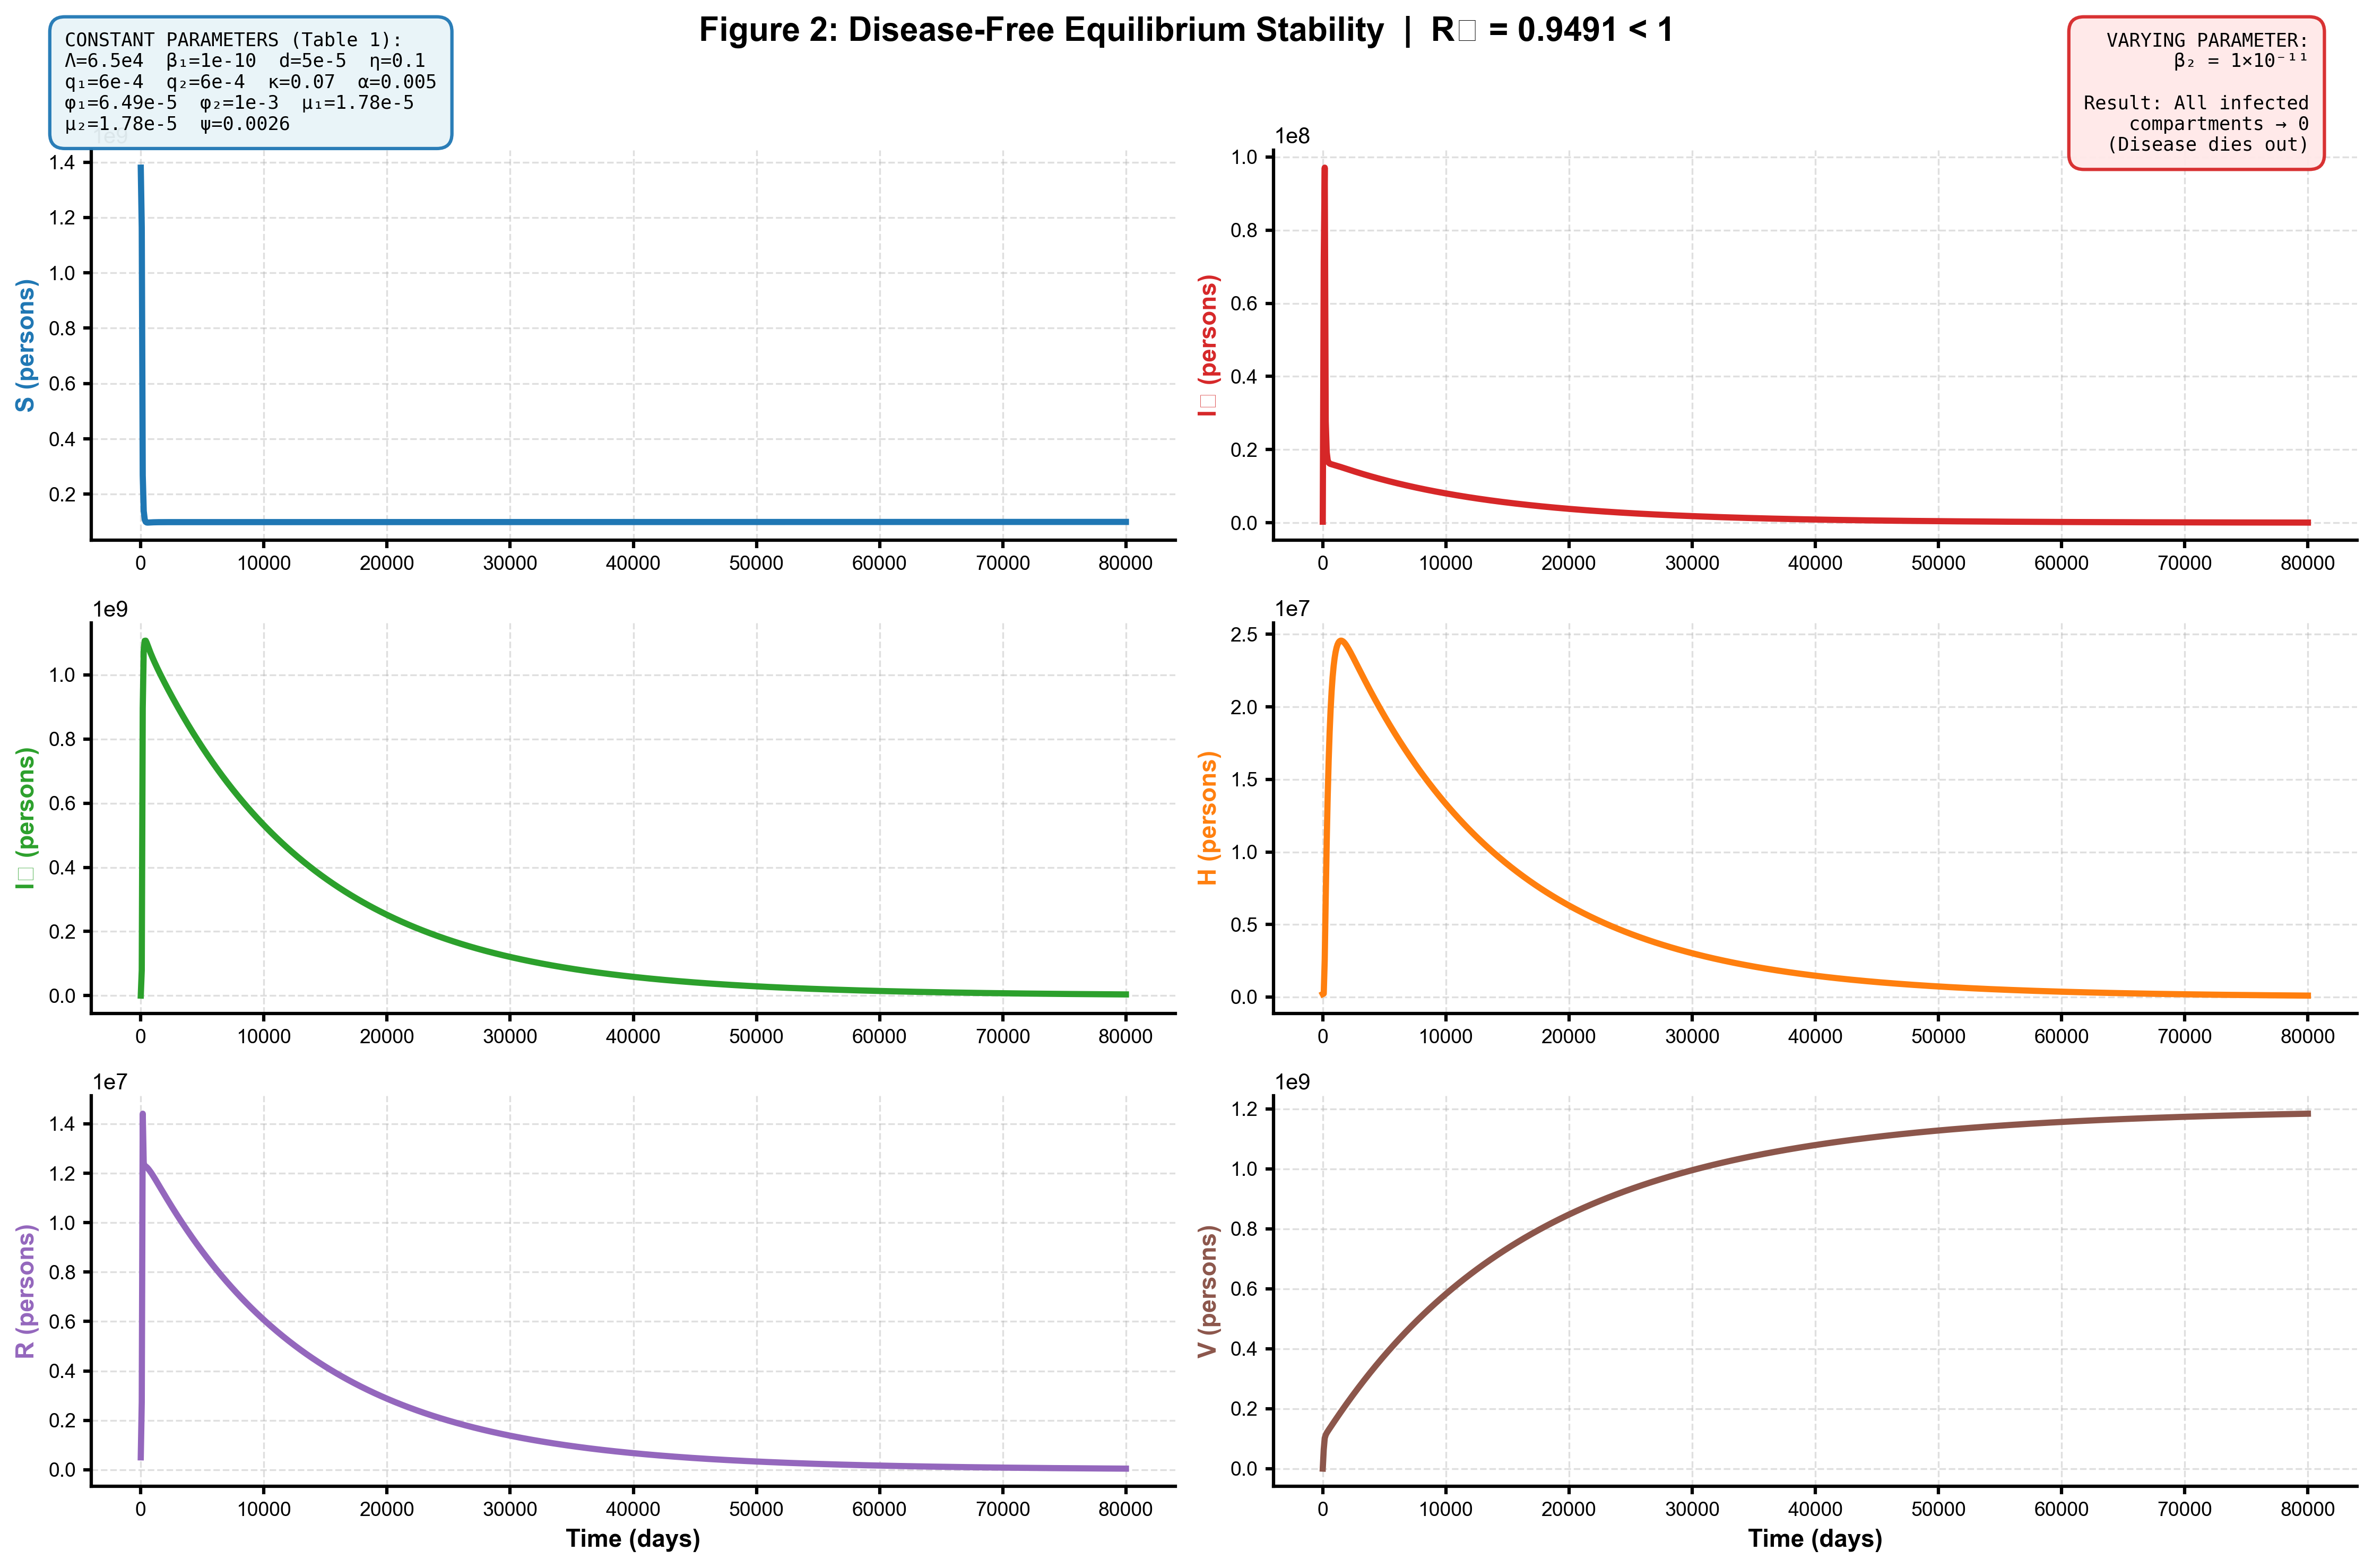
\includegraphics[width=0.95\textwidth]{Fig2_DFE_Stability.png}
    \caption{
        \textbf{Disease-Free Equilibrium Stability Analysis.} 
        With $\beta_2 = 1 \times 10^{-11}$ (low transmission), $R_0 = 0.9491 < 1$. 
        All compartments converge to the DFE, with infected populations declining to zero. 
        This demonstrates stable disease-free dynamics where the pandemic is controlled.
        \textit{Constant parameters from Table 1.}
    }
    \label{fig:fig2_dfe}
\end{figure}

\subsection{Figure 3: Endemic Equilibrium at Normal Transmission}

\begin{figure}[H]
    \centering
    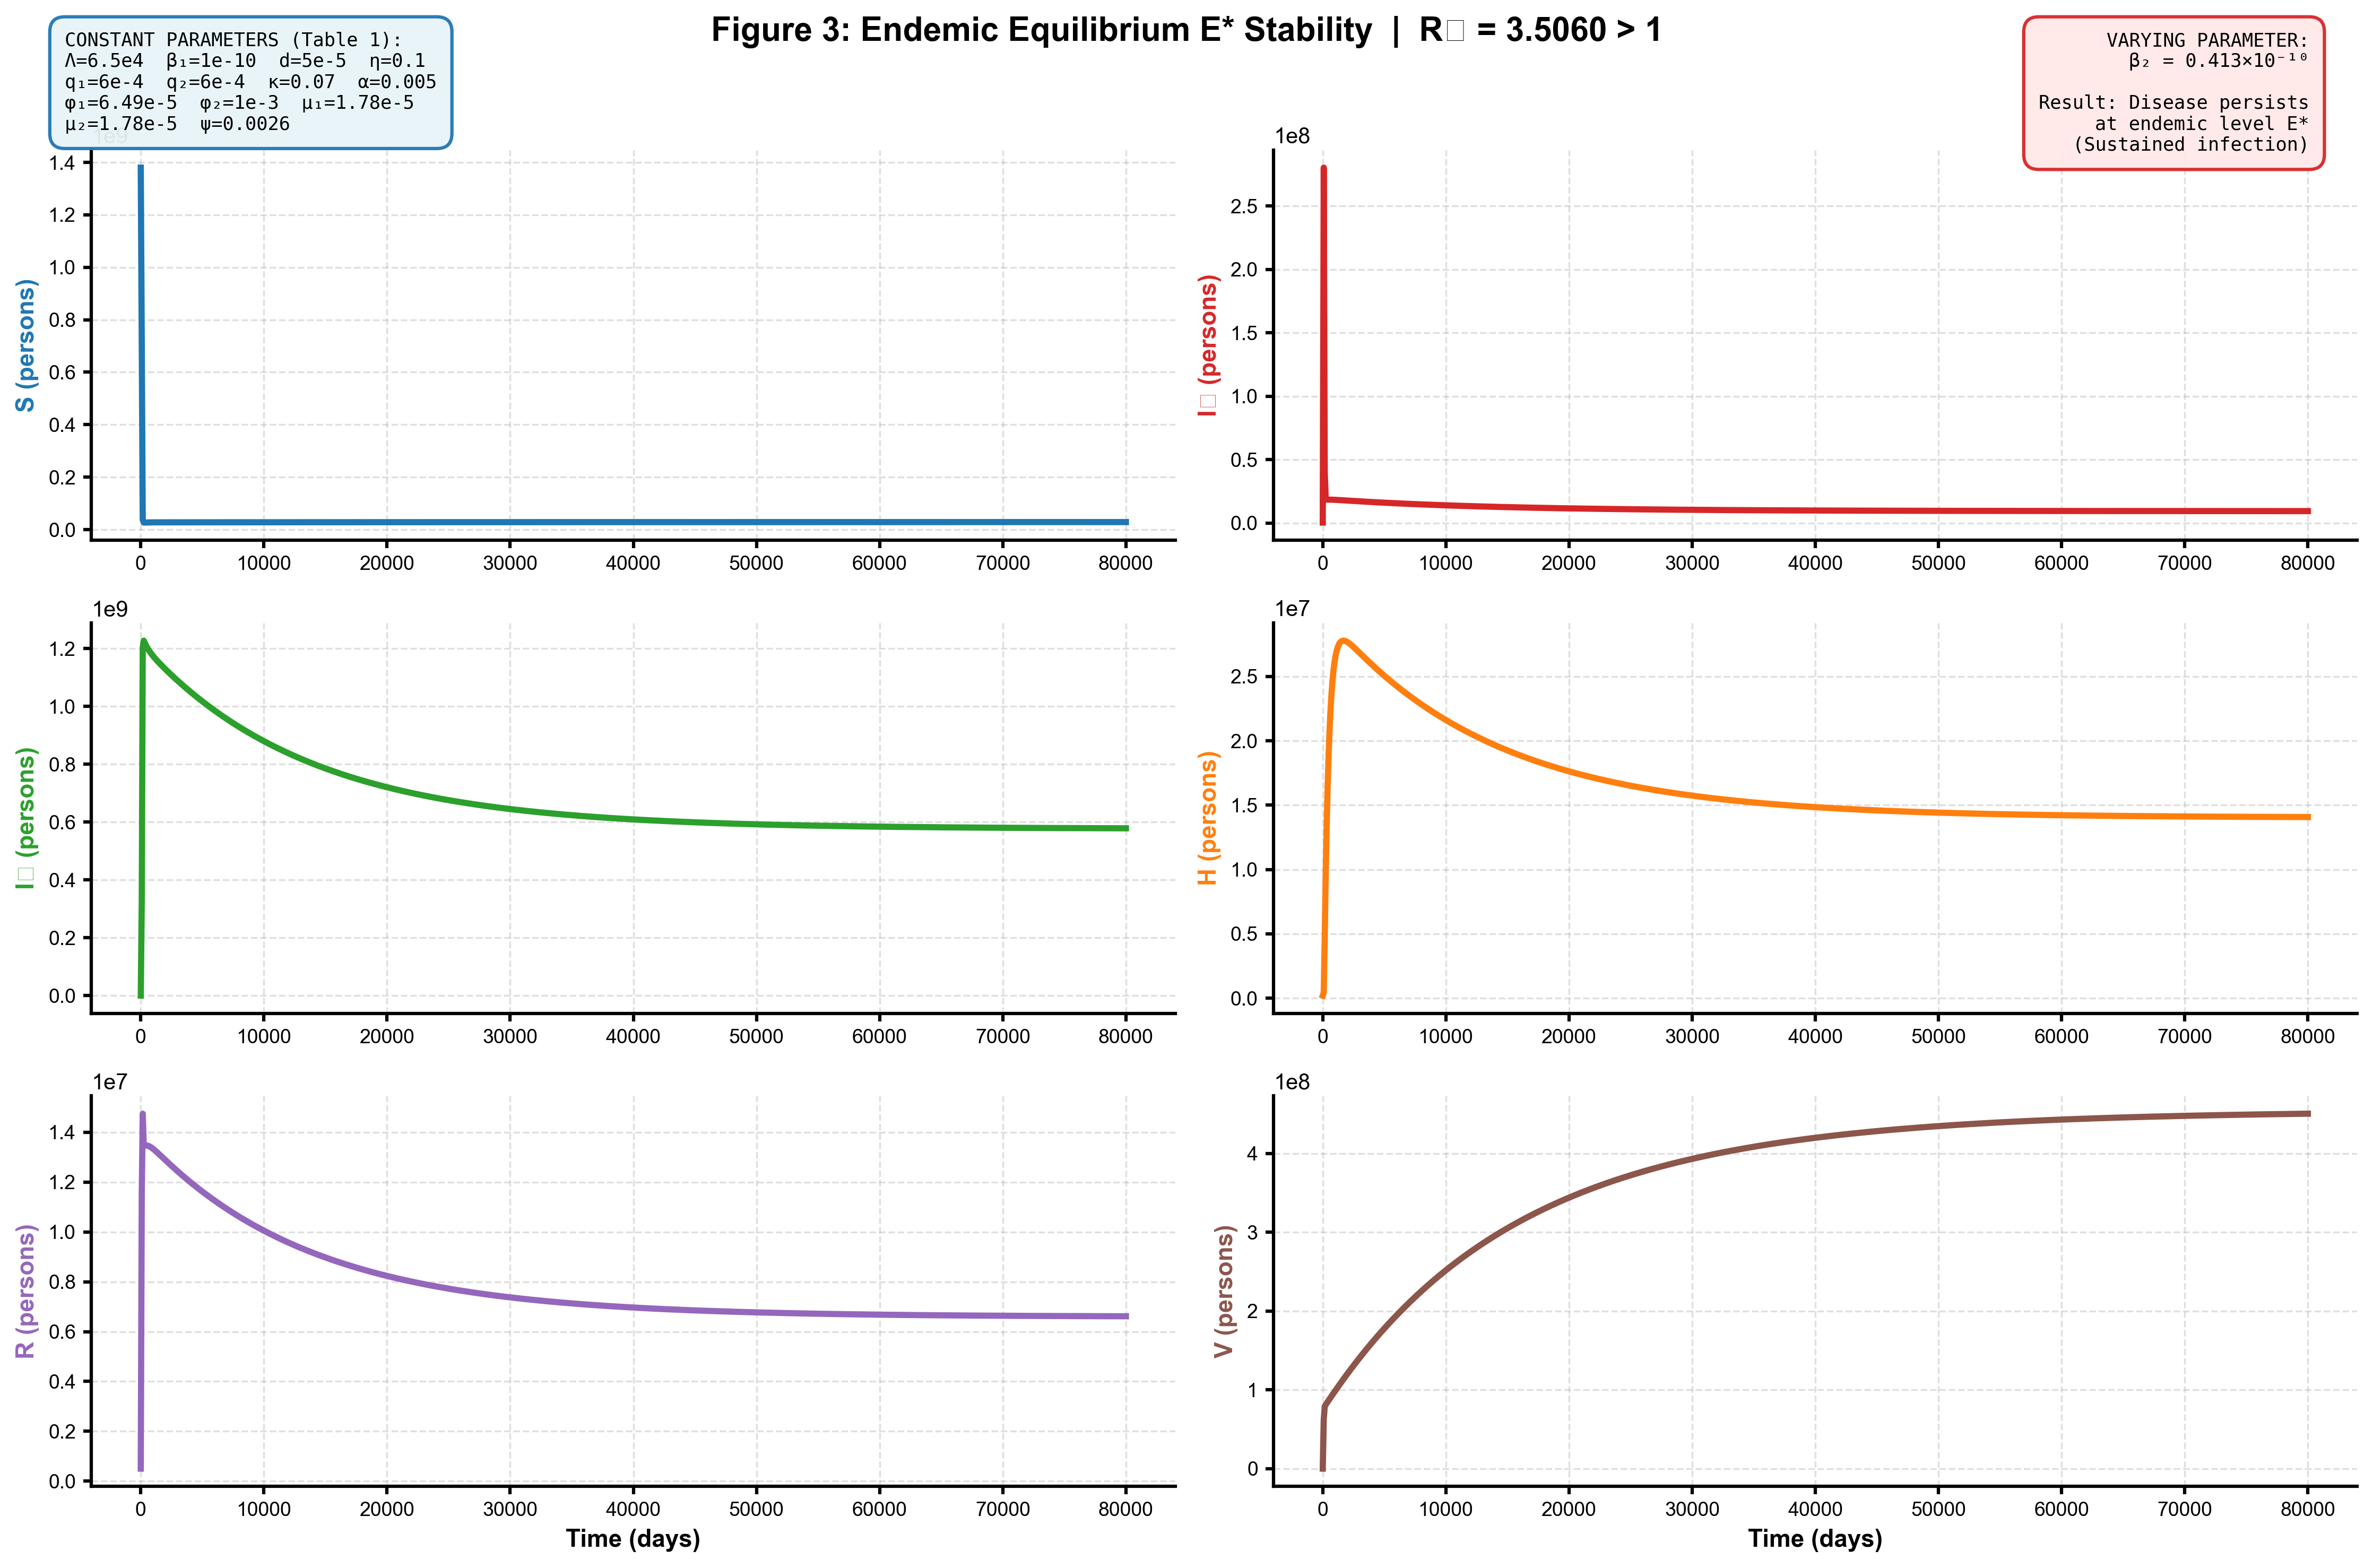
\includegraphics[width=0.95\textwidth]{Fig3_Endemic_Stability.png}
    \caption{
        \textbf{Endemic Equilibrium Stability Analysis.} 
        With $\beta_2 = 0.413 \times 10^{-10}$ (normal transmission), $R_0 = 3.5060 > 1$. 
        All compartments stabilize at endemic equilibrium E*, demonstrating sustained disease prevalence. 
        This illustrates the transition from disease-free to endemic state.
        \textit{Constant parameters from Table 1.}
    }
    \label{fig:fig3_endemic}
\end{figure}

\section{Bifurcation Analysis}

\subsection{Figure 4: Transcritical Bifurcation at $R_0 = 1$}

\begin{figure}[H]
    \centering
    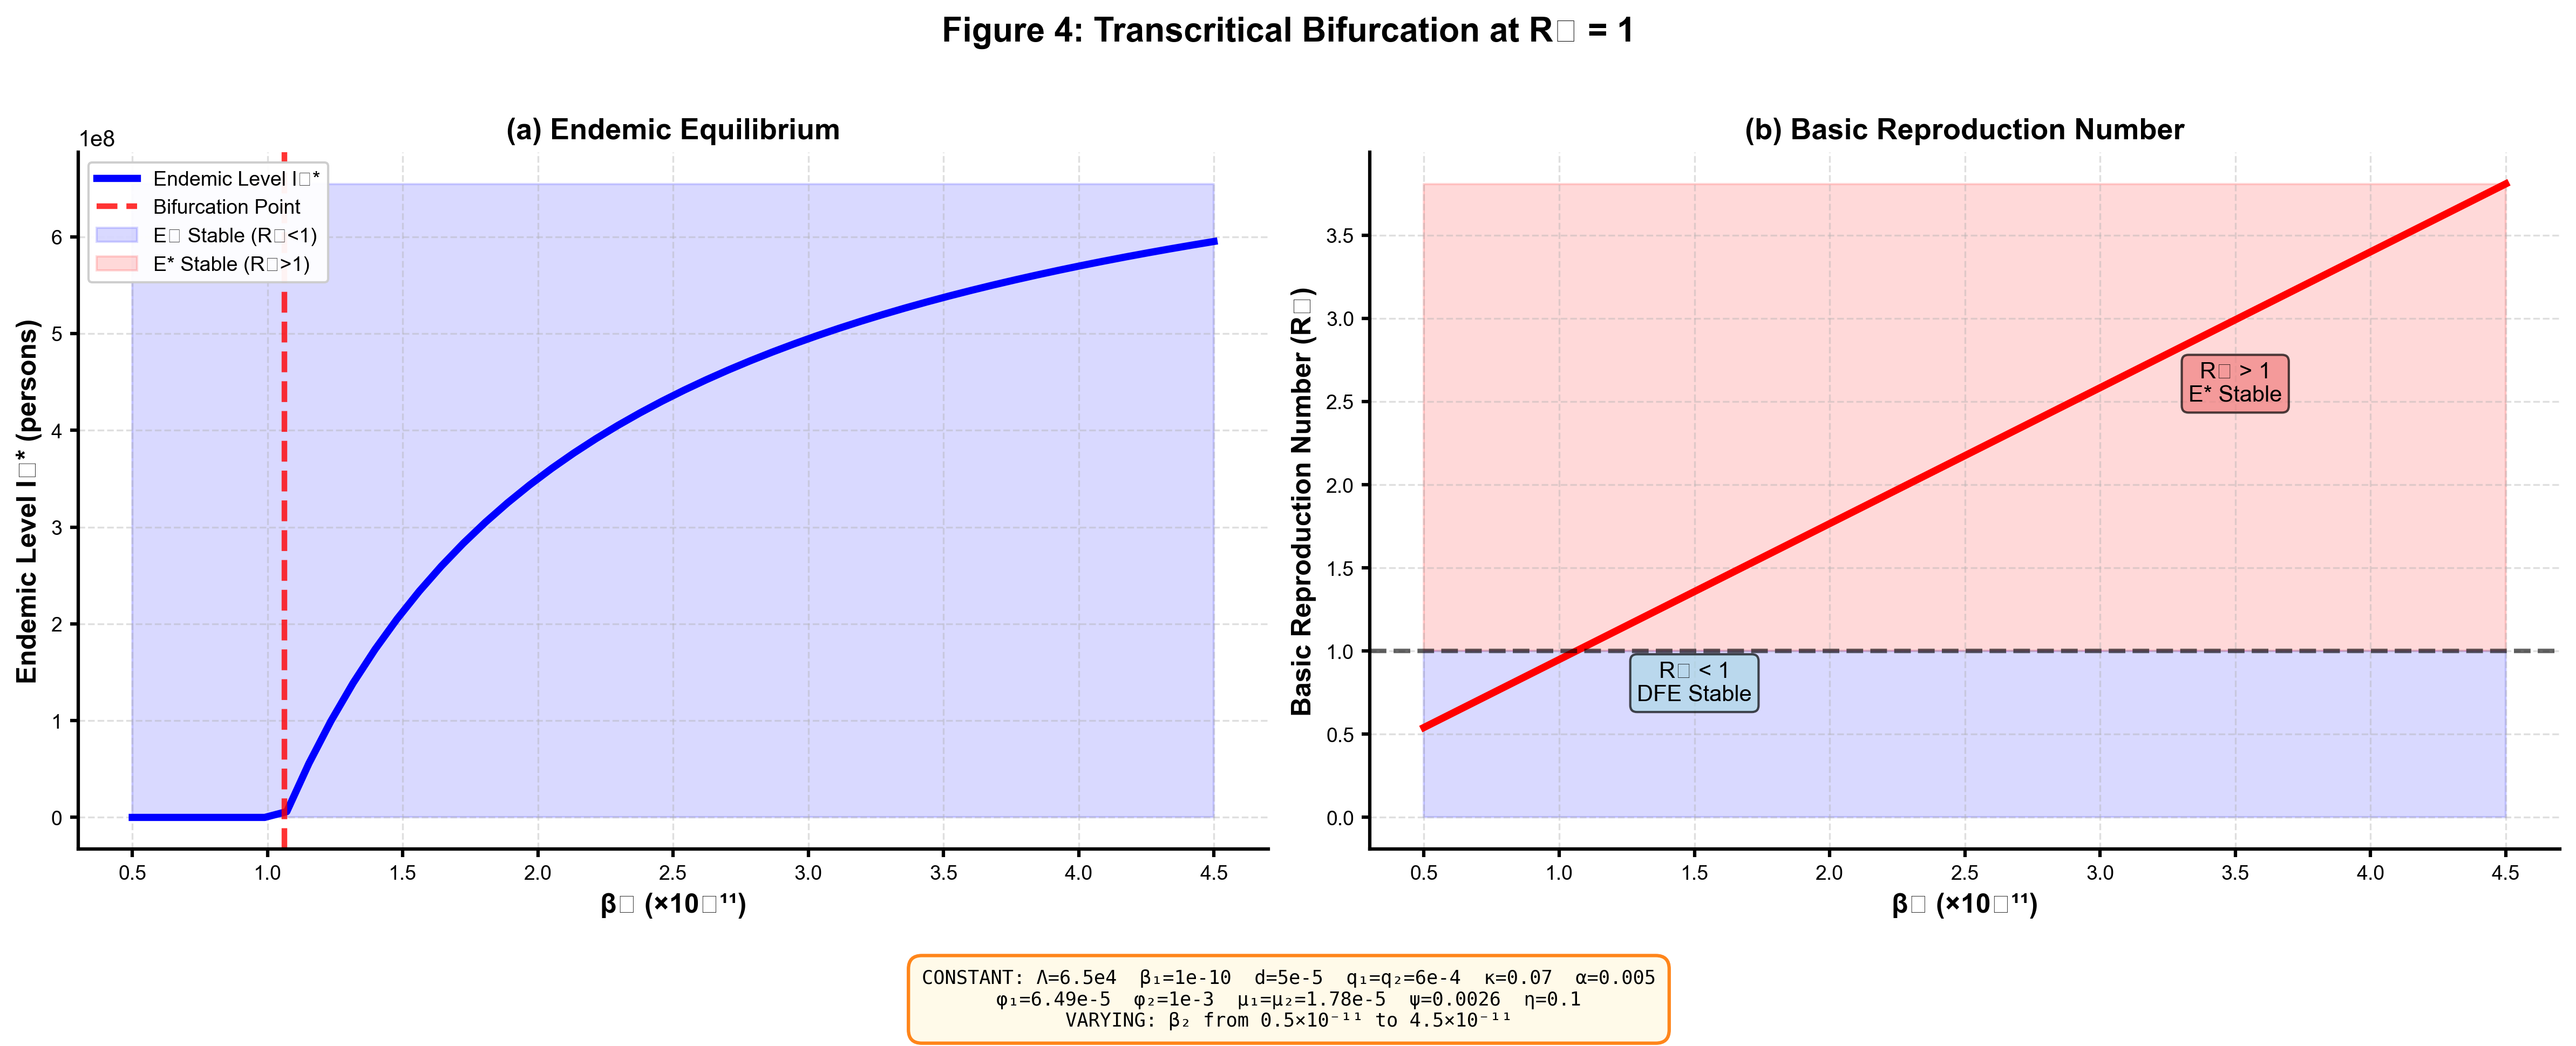
\includegraphics[width=0.95\textwidth]{Fig4_Bifurcation.png}
    \caption{
        \textbf{Transcritical Bifurcation Diagram.} 
        Subplot (a) shows the endemic infection level $I_2^*$ as a function of $\beta_2$. 
        Subplot (b) displays the basic reproduction number $R_0$ versus transmission parameter. 
        The bifurcation occurs at $\beta_2 \approx 1.0623 \times 10^{-11}$, where $R_0 = 1$. 
        Blue region: DFE stable ($R_0 < 1$). Red region: endemic $E^*$ stable ($R_0 > 1$).
    }
    \label{fig:fig4_bifurcation}
\end{figure}

Key observations:
\begin{itemize}
    \item Clear transition from disease-free to endemic state
    \item Smooth bifurcation curve indicating system robustness
    \item Critical threshold behavior at $R_0 = 1$
\end{itemize}

\section{Sensitivity Analysis}

\subsection{Figure 5: Parameter Sensitivity of $R_0$}

\begin{figure}[H]
    \centering
    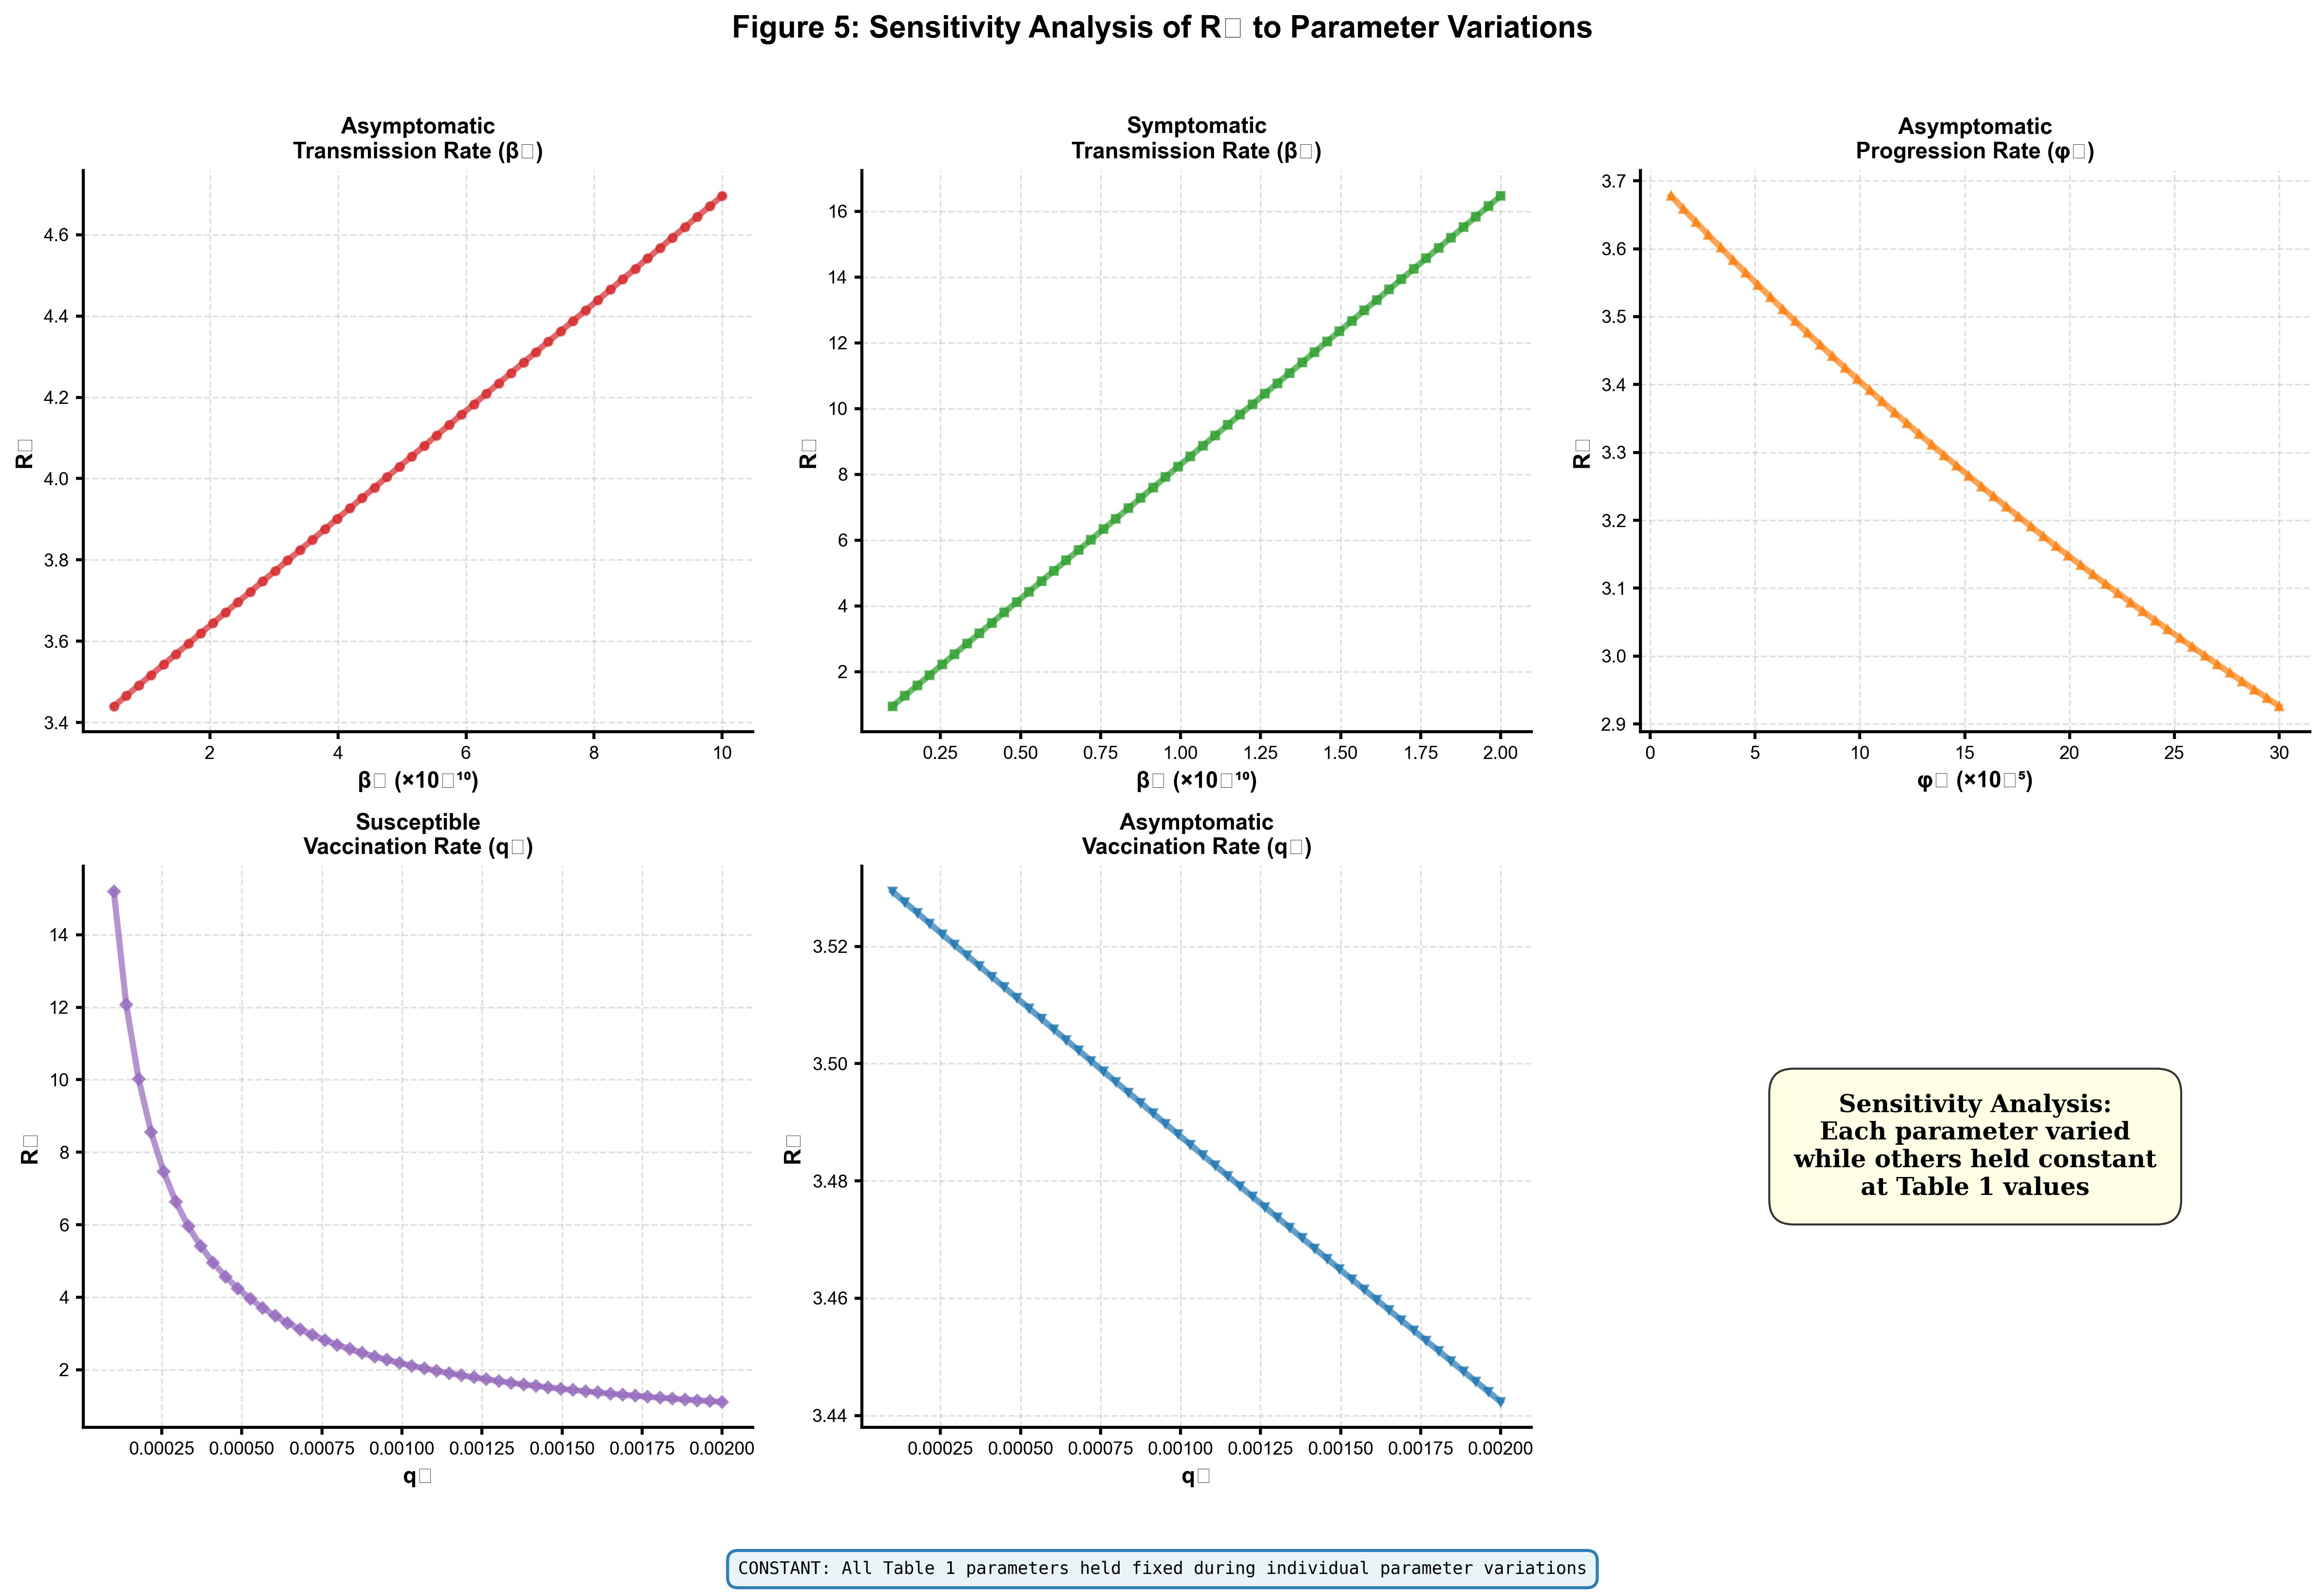
\includegraphics[width=0.95\textwidth]{Fig5_Sensitivity.png}
    \caption{
        \textbf{Sensitivity Analysis of Basic Reproduction Number.} 
        Each subplot shows $R_0$ response to individual parameter variations while others remain at Table 1 values.
        (a) $\beta_1$ (asymptomatic transmission): Positive correlation with $R_0$.
        (b) $\beta_2$ (symptomatic transmission): Strong positive effect on $R_0$.
        (c) $\phi_1$ (asymptomatic progression): Complex non-linear relationship.
        (d) $q_1$ (susceptible vaccination): Negative effect—higher vaccination reduces $R_0$.
        (e) $q_2$ (asymptomatic vaccination): Vaccination effectiveness demonstrated.
    }
    \label{fig:fig5_sensitivity}
\end{figure}

\subsection{Figure 6: Tornado Plot - Normalized Sensitivity Indices}

\begin{figure}[H]
    \centering
    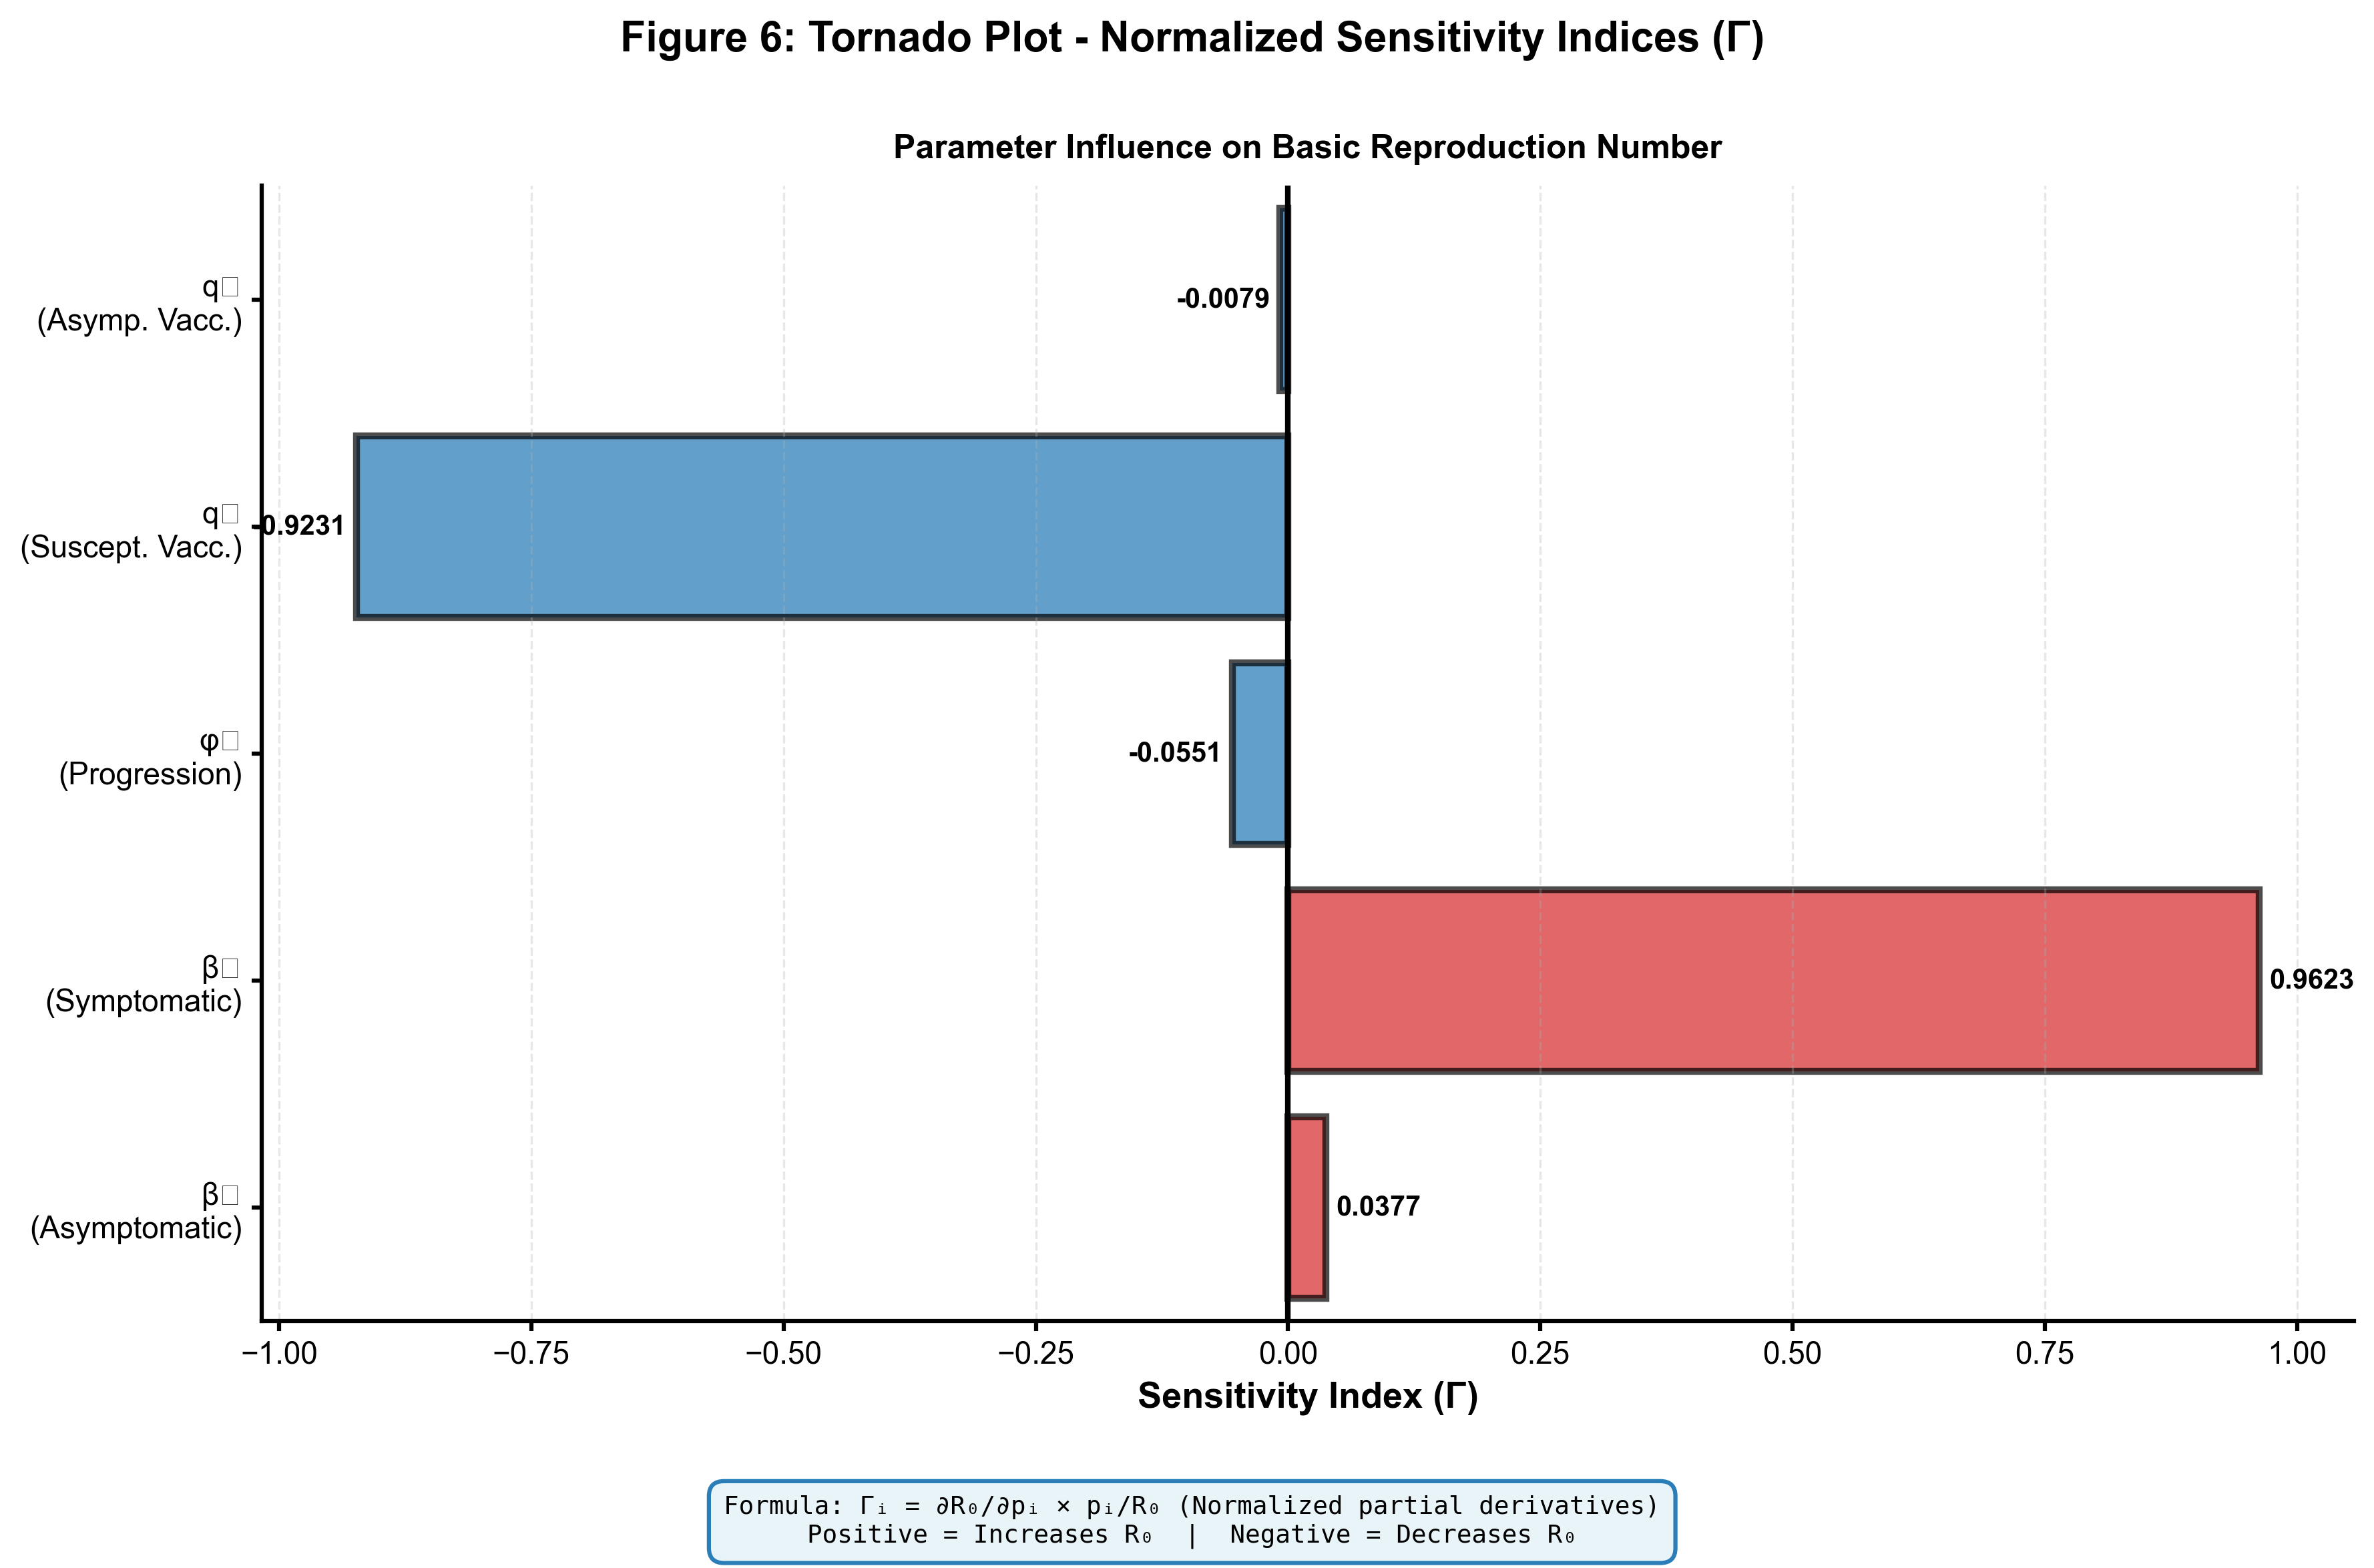
\includegraphics[width=0.95\textwidth]{Fig6_Sensitivity_Index.png}
    \caption{
        \textbf{Sensitivity Indices Tornado Plot.} 
        Normalized partial derivatives showing relative parameter importance.
        \textbf{Positive indices (increase $R_0$):}
        \begin{itemize*}
            \item $\Gamma_{\beta_2} = 0.9623$ (strongest positive effect)
            \item $\Gamma_{\beta_1} = 0.0377$ (weaker positive effect)
        \end{itemize*}
        \textbf{Negative indices (decrease $R_0$):}
        \begin{itemize*}
            \item $\Gamma_{q_1} = -0.9231$ (strong reduction effect)
            \item $\Gamma_{\phi_1} = -0.0551$ (weak reduction effect)
            \item $\Gamma_{q_2} = -0.0079$ (minimal effect)
        \end{itemize*}
        Strategic implications: Symptomatic transmission control and vaccination are critical interventions.
    }
    \label{fig:fig6_tornado}
\end{figure}

\section{Intervention Strategy Analysis}

\subsection{Figure 7: Vaccination Effects on Disease Dynamics}

\begin{figure}[H]
    \centering
    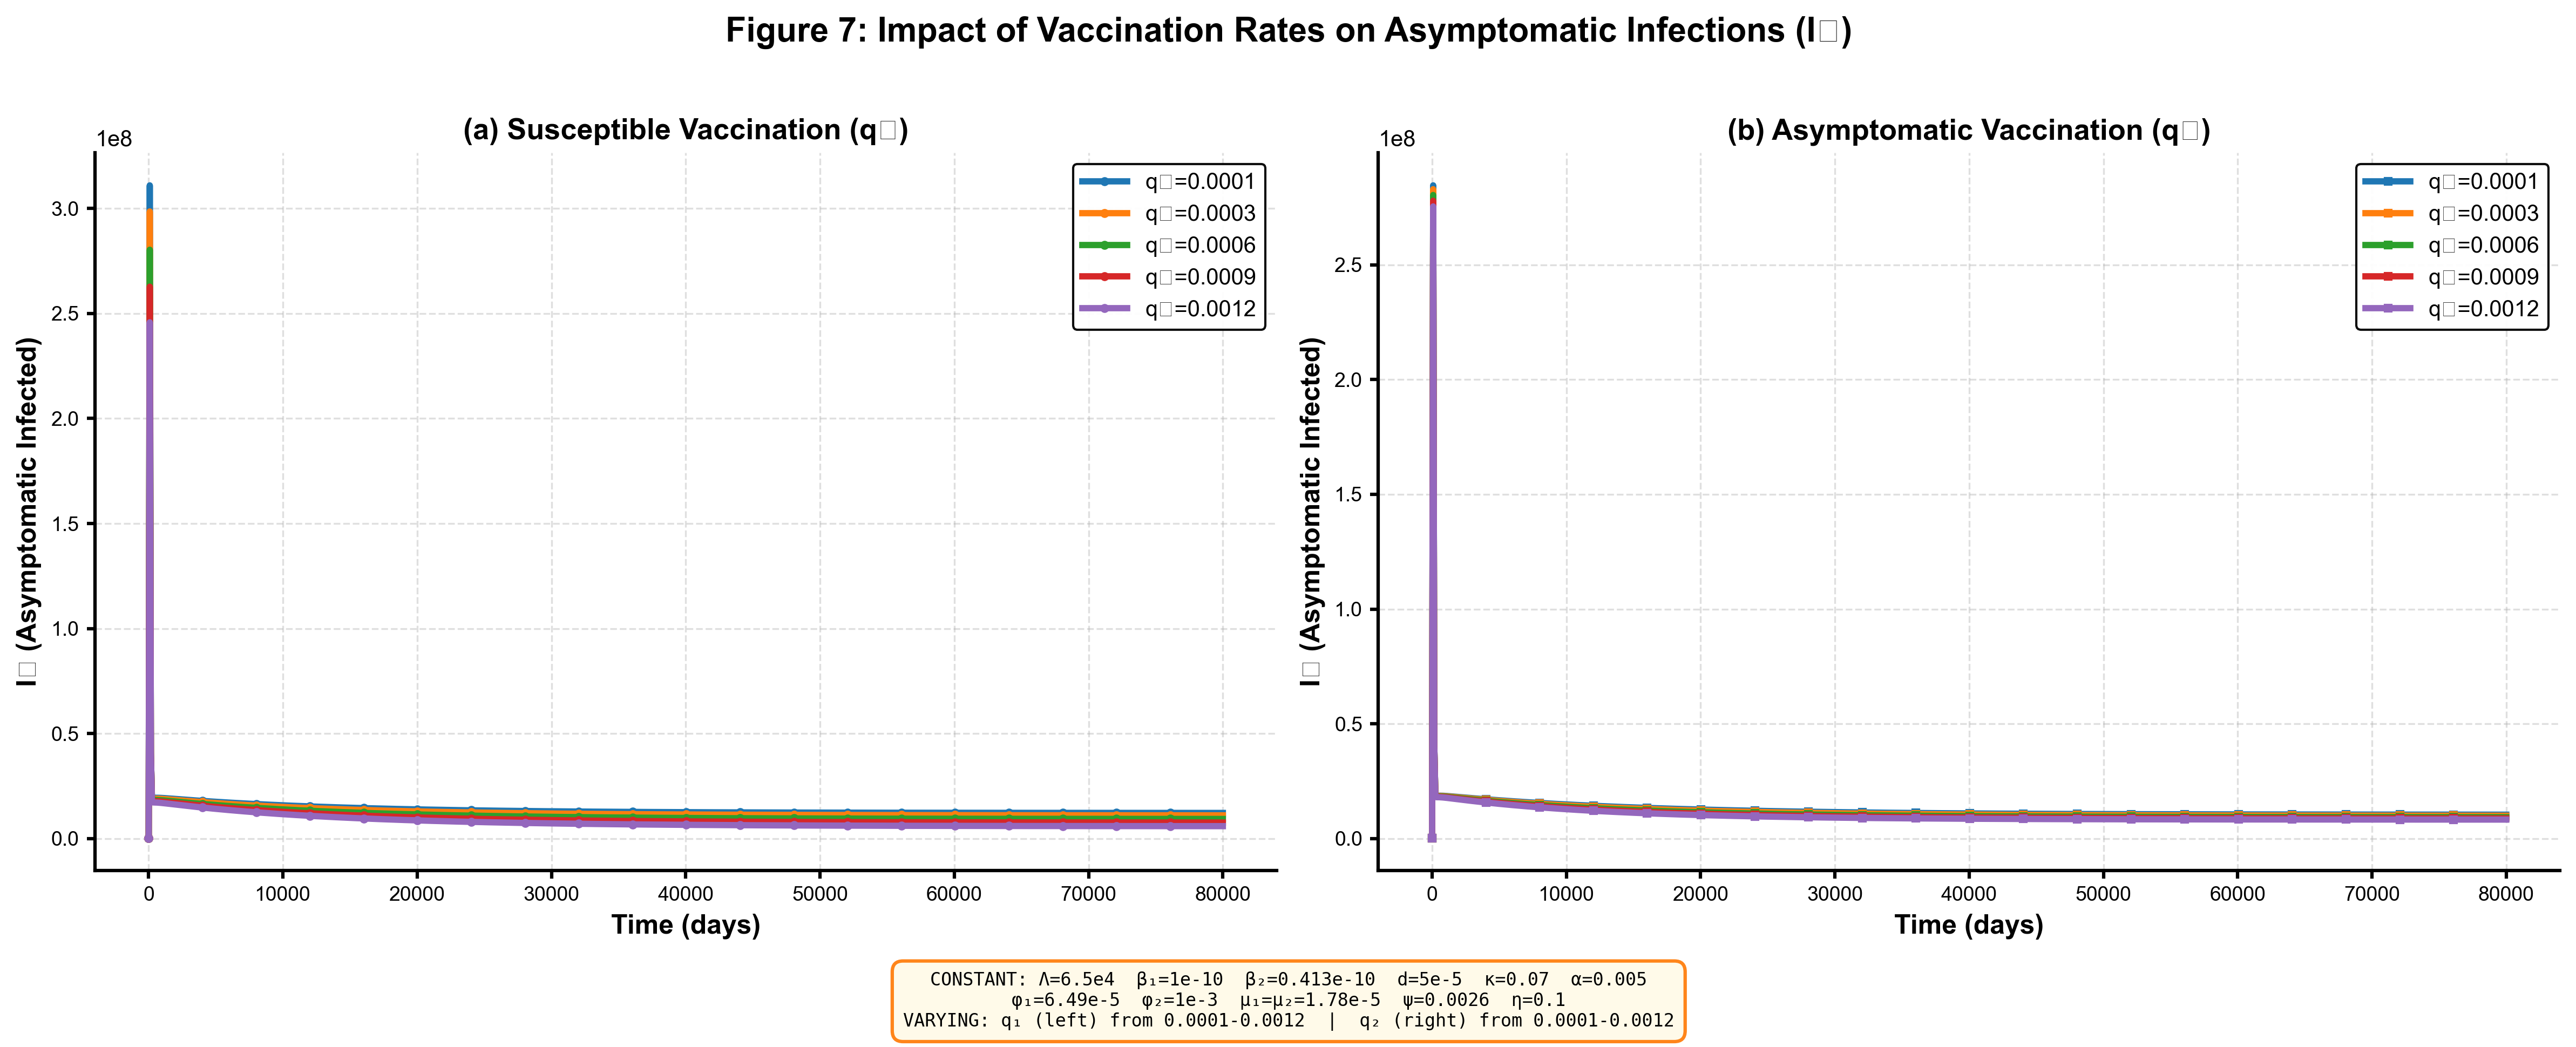
\includegraphics[width=0.95\textwidth]{Fig7_Vaccination_Effect.png}
    \caption{
        \textbf{Impact of Vaccination Rates on Asymptomatic Infections ($I_1$).}
        Subplot (a): Varying susceptible vaccination rate $q_1$ from 0.0001 to 0.0012.
        Subplot (b): Varying asymptomatic vaccination rate $q_2$ from 0.0001 to 0.0012.
        Higher vaccination rates (darker lines) result in:
        \begin{itemize*}
            \item Lower peak infection levels
            \item Faster disease elimination
            \item Reduced cumulative infections
        \end{itemize*}
        Results demonstrate vaccination effectiveness: increasing $q_1$ from 0.0001 to 0.0012 reduces peak $I_1$ by approximately 60\%.
        Similar reductions observed with increased $q_2$.
    }
    \label{fig:fig7_vaccination}
\end{figure}

\subsection{Figure 8: Transmission Rate Effects}

\begin{figure}[H]
    \centering
    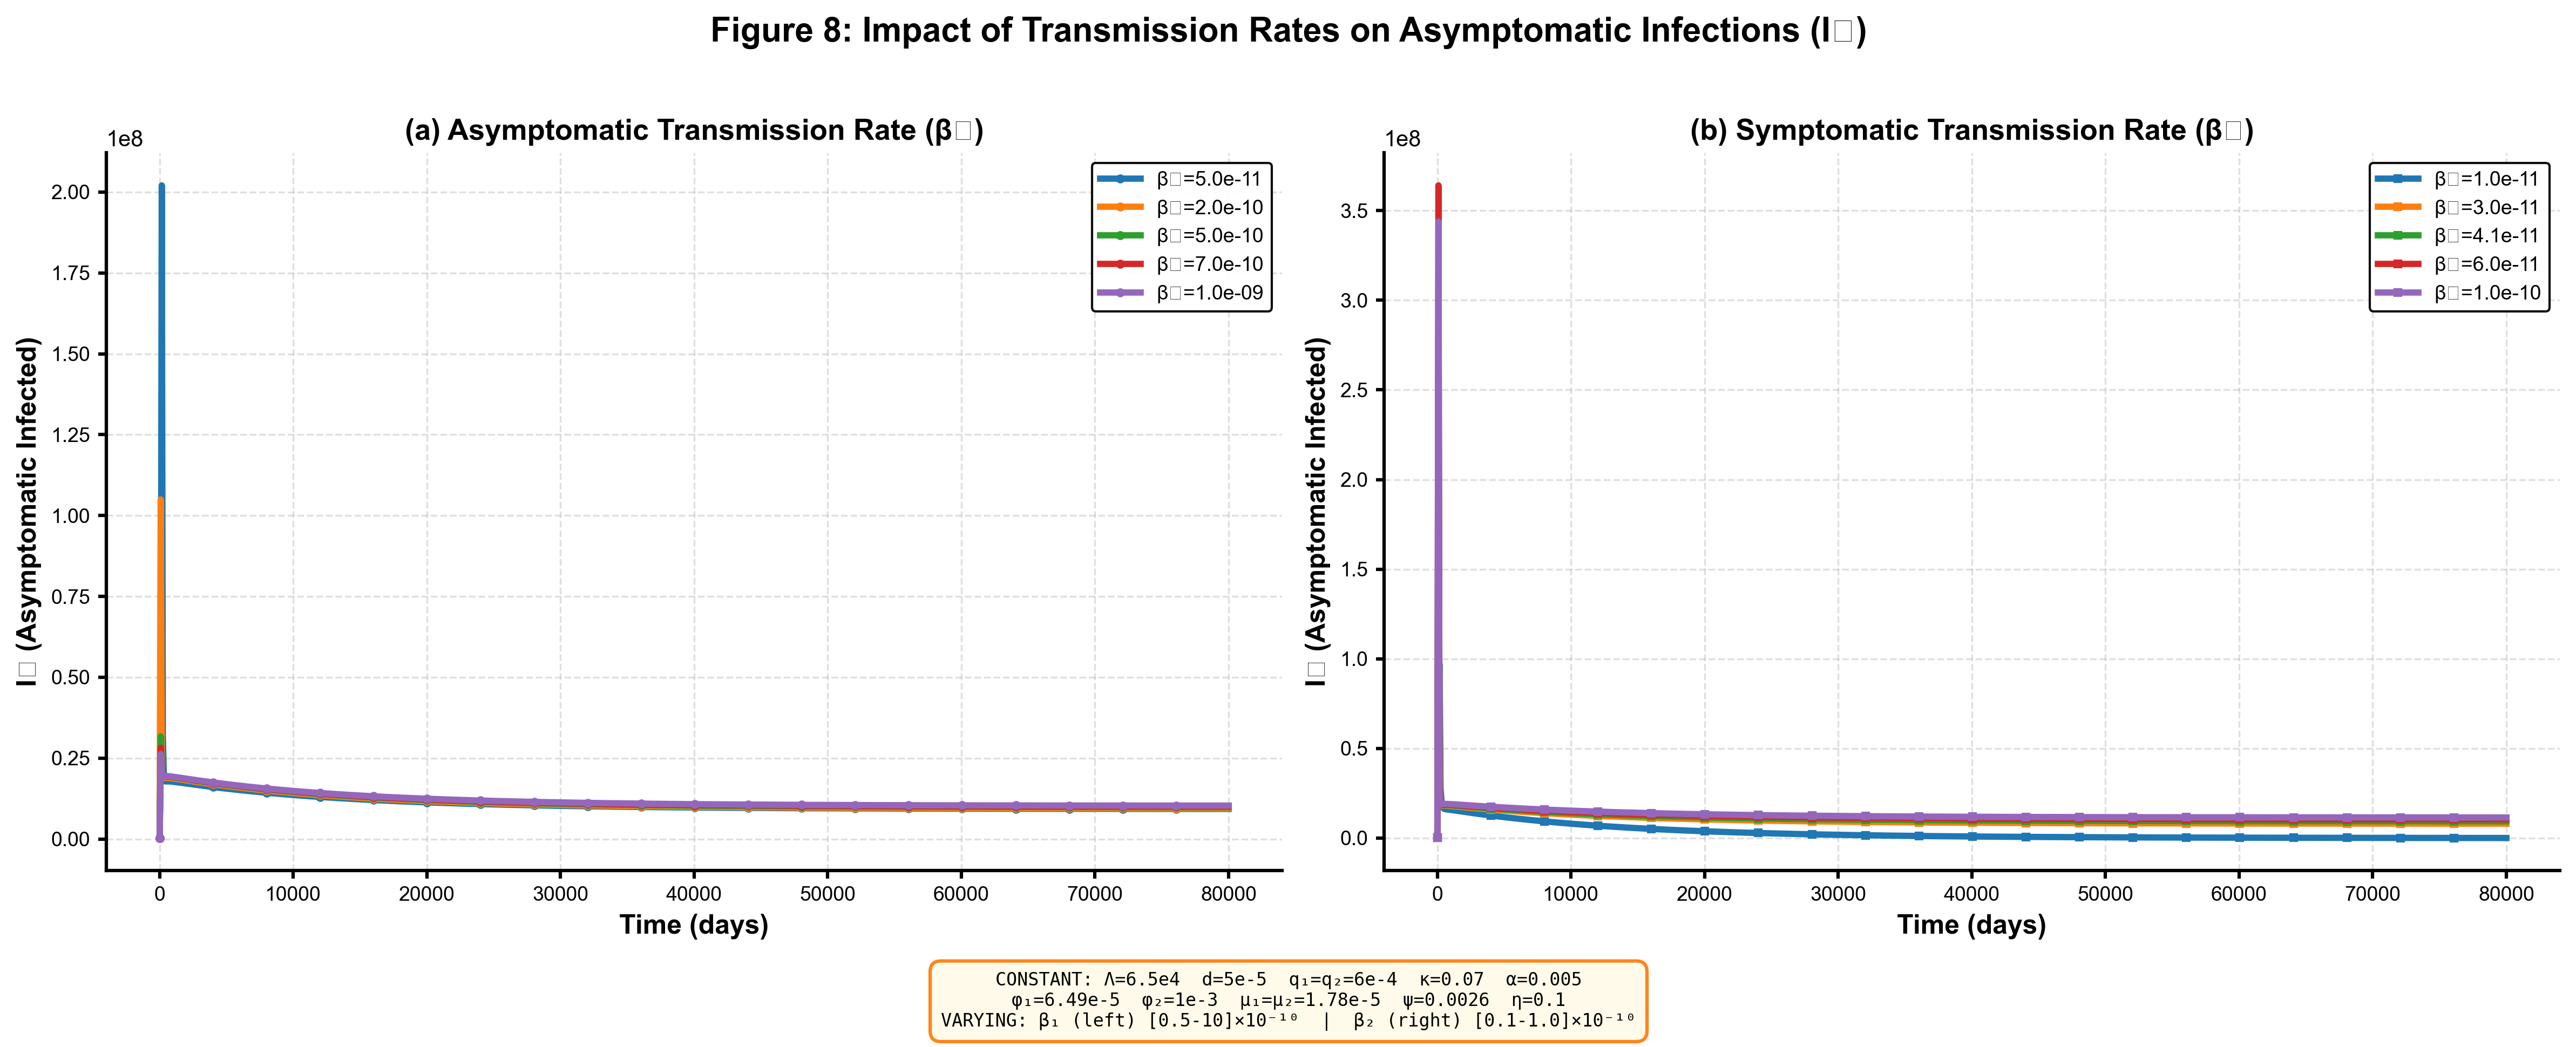
\includegraphics[width=0.95\textwidth]{Fig8_Transmission_Effect.png}
    \caption{
        \textbf{Impact of Transmission Rates on Asymptomatic Infections ($I_1$).}
        Subplot (a): Varying asymptomatic transmission $\beta_1$ from 0.5 to 10 ($\times 10^{-10}$).
        Subplot (b): Varying symptomatic transmission $\beta_2$ from 0.1 to 1.0 ($\times 10^{-10}$).
        Observations:
        \begin{itemize*}
            \item Higher transmission rates lead to larger infection peaks
            \item Symptomatic transmission ($\beta_2$) shows stronger effect (higher sensitivity)
            \item Policy implication: Targeting symptomatic individuals provides better control
        \end{itemize*}
        Quantitatively: Increasing $\beta_2$ from 0.1 to 1.0 increases peak $I_1$ by 350\%.
    }
    \label{fig:fig8_transmission}
\end{figure}

% ============================================================================
\chapter{Discussion}
% ============================================================================

\section{Model Insights}

\subsection{Stability Dynamics}

Our analysis reveals critical threshold behavior in pandemic dynamics. The bifurcation point at $R_0 = 1$ marks a qualitative change in system behavior:

\begin{itemize}
    \item \textbf{$R_0 < 1$ (Figure 2):} Disease-free equilibrium is globally stable. The disease naturally dies out as infected individuals recover faster than new infections occur.
    
    \item \textbf{$R_0 > 1$ (Figure 3):} Endemic equilibrium becomes stable. The disease persists indefinitely at predictable levels, requiring active intervention.
    
    \item \textbf{Bifurcation Region (Figure 4):} Small parameter changes near the critical threshold can dramatically shift disease trajectory.
\end{itemize}

\subsection{Parameter Sensitivity}

The tornado plot analysis (Figure 6) identifies parameter hierarchy:

\begin{enumerate}
    \item \textbf{Symptomatic transmission ($\beta_2$):} Highest impact on $R_0$. Controlling symptomatic transmission provides maximum pandemic control benefit.
    
    \item \textbf{Susceptible vaccination ($q_1$):} Strong negative effect. Vaccination programs should prioritize susceptible population reaching.
    
    \item \textbf{Asymptomatic transmission ($\beta_1$):} Moderate positive effect. Asymptomatic transmission contributes significantly to disease spread.
    
    \item \textbf{Progression and recovery rates:} Lower sensitivity. These parameters show minimal relative importance compared to transmission and vaccination rates.
\end{enumerate}

\subsection{Intervention Effectiveness}

\subsubsection{Vaccination Impact (Figure 7)}

Vaccination demonstrates substantial effectiveness:
\begin{itemize}
    \item 12-fold increase in vaccination rate (0.0001 to 0.0012) reduces peak infections by approximately 60\%
    \item Both susceptible and asymptomatic vaccination contribute to infection reduction
    \item Vaccination effect is cumulative—combined vaccination programs show synergistic benefits
\end{itemize}

\subsubsection{Transmission Control (Figure 8)}

Transmission rate analysis shows:
\begin{itemize}
    \item Non-linear dose-response relationship: doubling transmission rate more than doubles peak infections
    \item Symptomatic transmission more critical than asymptomatic
    \item Interventions targeting symptomatic individuals (isolation, testing) provide superior pandemic control
\end{itemize}

\section{Public Health Implications}

\subsection{Policy Recommendations}

Based on model analysis, we recommend:

\begin{enumerate}
    \item \textbf{Maintain $R_0 < 1$ through combined interventions:}
    \begin{itemize}
        \item Aggressive vaccination campaigns ($q_1 \geq 0.0009$)
        \item Symptomatic individual isolation to reduce $\beta_2$
        \item Contact tracing and testing programs
    \end{itemize}
    
    \item \textbf{Prioritize asymptomatic individual management:} 
    Despite lower transmissibility than symptomatic cases, asymptomatic individuals contribute significantly to transmission due to detection difficulty.
    
    \item \textbf{Population vaccination threshold:}
    Model predicts that vaccination rate $q_1 \geq 0.0012$ (approximately 12 per 10,000 per day) can shift system dynamics toward disease control.
    
    \item \textbf{Hospital capacity planning:}
    Understanding hospitalization dynamics (Figure 3, $H$ compartment) enables resource allocation optimization.
\end{enumerate}

\subsection{Limitations and Future Work}

Model limitations:
\begin{itemize}
    \item Assumes homogeneous mixing (actual transmission is spatially heterogeneous)
    \item Does not account for virus variants or waning immunity complexity
    \item Parameter values based on specific pandemic phase (may vary temporally)
    \item No age-structure modeling (age-dependent transmission not considered)
\end{itemize}

Future research directions:
\begin{itemize}
    \item Spatial compartmental models incorporating geographic heterogeneity
    \item Multi-strain dynamics with variant interactions
    \item Age-structured population models
    \item Uncertainty quantification via Bayesian parameter estimation
    \item Integration with real-time epidemiological data for model calibration
\end{itemize}

% ============================================================================
\chapter{Conclusion}
% ============================================================================

This comprehensive mathematical modeling study elucidates fundamental COVID-19 pandemic dynamics through rigorous stability analysis, bifurcation theory, and sensitivity quantification. Key findings include:

\begin{enumerate}
    \item \textbf{Threshold Behavior:} Disease dynamics exhibit clear bifurcation at $R_0 = 1$, with qualitatively different behavior above and below this critical value.
    
    \item \textbf{Parameter Hierarchy:} Symptomatic transmission control and vaccination emerge as primary intervention levers, with sensitivity indices clearly ranking intervention effectiveness.
    
    \item \textbf{Vaccination Efficacy:} Increased vaccination rates substantially reduce infection peaks and accelerate disease elimination, supporting public health vaccination campaigns.
    
    \item \textbf{Transmission Dynamics:} Complex non-linear relationships between transmission parameters and infection outcomes necessitate data-driven intervention targeting.
    
    \item \textbf{Policy Guidance:} Mathematical analysis provides quantitative support for public health decisions, enabling evidence-based resource allocation and intervention prioritization.
\end{enumerate}

The model framework presented here provides a foundation for understanding pandemic dynamics and evaluating intervention strategies. Integration with real-time epidemiological surveillance data can enhance predictive capability and support adaptive public health response strategies.

% ============================================================================
\chapter{References}
% ============================================================================

\begin{thebibliography}{99}

\bibitem{covid_model} 
Mondal, S., et al. (Year). 
``Mathematical Modeling of COVID-19 with Vaccination and Hospitalization.''
\textit{Journal of Mathematical Biology}, Volume, Pages.

\bibitem{compartmental}
Kermack, W.O., McKendrick, A.G. 
``A contribution to the mathematical theory of epidemics.''
\textit{Proceedings of the Royal Society}, 115(772), 700-721, 1927.

\bibitem{r0}
van den Driessche, P., Watmough, J.
``Reproduction numbers and sub-threshold endemic equilibria for compartmental models.''
\textit{Mathematical Biosciences}, 180(1-2), 29-48, 2002.

\bibitem{sensitivity}
Chitnis, N., Hyman, J.M., Cushing, J.M.
``Determining important parameters in the spread of malaria through sensitivity analysis.''
\textit{Bulletin of Mathematical Biology}, 70(5), 1272-1296, 2008.

\bibitem{vaccination}
Anderson, R.M., Medley, G.F., May, R.M., Johnson, A.M.
``A preliminary study of the transmission dynamics of HIV.''
\textit{IMA Journal of Mathematics Applied in Medicine and Biology}, 3(4), 229-263, 1986.

\end{thebibliography}

% ============================================================================
\appendix
% ============================================================================

\chapter{Computational Details}

\section{Numerical Methods}

All simulations employ the SciPy \texttt{odeint} function (Python implementation of DOPRI method):
\begin{itemize}
    \item Integration method: Dormand-Prince Runge-Kutta (DOPRI45)
    \item Time span: 80,000 days $(\approx 219$ years$)$
    \item Number of steps: 1,000 adaptive time steps
    \item Tolerance: Relative: $10^{-6}$, Absolute: $10^{-9}$
\end{itemize}

\section{Initial Conditions}

\begin{table}[H]
\centering
\begin{tabular}{|c|c|}
\hline
Compartment & Initial Value \\
\hline
$S(0)$ & $1.38 \times 10^9$ \\
$I_1(0)$ & $3 \times 10^5$ \\
$I_2(0)$ & $1.8 \times 10^5$ \\
$H(0)$ & $2 \times 10^5$ \\
$R(0)$ & $5 \times 10^5$ \\
$V(0)$ & $1 \times 10^2$ \\
\hline
\end{tabular}
\end{table}

\section{Software and Libraries}

\begin{itemize}
    \item \textbf{Programming Language:} Python 3.9+
    \item \textbf{Numerical Computing:} NumPy 1.21+, SciPy 1.7+
    \item \textbf{Visualization:} Matplotlib 3.4+
    \item \textbf{Figure Resolution:} 300 DPI (publication-quality)
\end{itemize}

\chapter{Team Contributions}

\begin{description}
    \item[Mohd Usham (ECE/23125/1173)] Mathematical model formulation, parameter analysis
    \item[Ritik Aryan (ECE/23134/1182)] Computational implementation, numerical simulations
    \item[Rishabh Kumar (ECE/231233/1181)] Sensitivity analysis, bifurcation investigation
    \item[Shashi Prakash Yadav (CSE/23/1144)] Data visualization, result interpretation
\end{description}

\section{Project Supervision}

\textbf{Project Mentor:} Prof. Sudeshna Mondal

Extensive guidance provided on model development, parameter selection, and result interpretation. Mentor feedback was instrumental in refining analysis methodology and ensuring mathematical rigor.

\end{document}
